\section{Kevin Natanael Nainggolan(1174059)}

\subsection{Instalasi Map Server}
\begin{enumerate}
    \item Download terlebih dahulu map servernya. Untuk webnya bisa \href{https://mapserver.org/}{Klik disini} atau \href{https://ms4w.com/}{Klik disini} Untuk windows.
	\item Untuk bagian yang mendownload versi zip, bisa langsung extract setelah download.
	\item Buka folder dengan nama ms4w/Apache/cgi-bin.
	\item Copy semua yang ada pada folder cgi-bin.
	\item Masuk ke directory C:/xampp/cgi-bin pada komputer masing-masing.
	\item Paste di dalamnya semua.
	\item Lakukan test pada localhost masing-masing.
	\item Aktifkan juga xampp masing-masing agar dapat mengakses localhost.
	\item Masukan localhost/cgi-bin/mapserv.exe pada browser masing-masing, dan hasilnya akan seperti dibawah.
	
	\hfill\break
    \begin{figure}[H]
		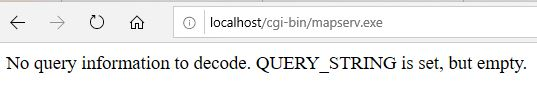
\includegraphics[width=12cm]{figures/1174059/tugas4/1.jpg}
		\centering
		\caption{Tampilan uji coba mapserver}
    \end{figure}
    \hfill\break
	
	\item Gambar di atas menujukan bahwa mapservernya sudah dapat digunakan hanya saja tidak ada file dengan exitensi .map yang dieksekusi
	\item Setelah itu lanjut dengan menginstal MapProxy
	\item Ketikan saja pip install mapproxy pada cmd di komputer masing-masing, bila sudah pernah menginstal sebelumnya akan tampil seperti berikut
	
	\hfill\break
    \begin{figure}[H]
		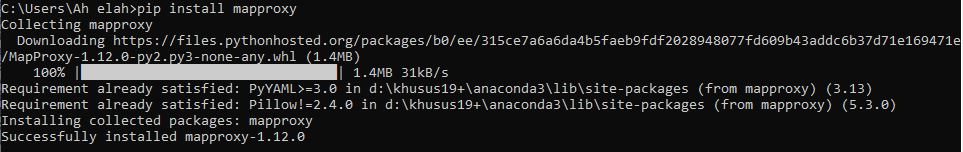
\includegraphics[width=12cm]{figures/1174059/tugas4/mapproxy.jpg}
		\centering
		\caption{Install mapproxy}
    \end{figure}
    \hfill\break
\end{enumerate}

\subsection{Link Youtube}
\href{https://youtu.be/y4RwhtPPur8}{Klik disini}